\chapter{Modelagem Utilizando Operadores Diferenciais}\label{cap_mod_od}

\thispagestyle{empty}

\markboth{Modelagem Utilizando Operadores Diferenciais}{Operadores de Laplace-Beltrami e Reconstrução de Superfícies Lineares por Partes}

\section{Modelagem geométrica}\label{LB_Int}
%%%%%%%%%%%%%%%%%%%%%%%%%%%%% SLIDE 4.0 %%%%%%%%%%%%%%%%%%%%%%%%%%%%%%%%%%%%%%%%%%%
\begin{frame}{{\bf \color{blue} Modelagem geométrica}}

\begin{block}{\bf Modelagem geométrica}
Conjunto de técnicas e algoritmos utilizados para modelar determinadas formas matemáticas, sujeitas a condições particulares de forma e suavidade.

\medskip

Utilizado em especial em CAD/CAM \textit{(computer aided design / manufacturing)}, por seu alto poder em modelagem de superfícies.

\medskip

Uma forma possível de se modelar é com a utilização da \destaq{discretização do operador de Laplace-Beltrami}.
\end{block}

\end{frame}

%%%%%%%%%%%%%%%%%%%%%%%%%%%%% SLIDE 4.1 %%%%%%%%%%%%%%%%%%%%%%%%%%%%%%%%%%%%%%%%%%%
\begin{frame}{{\bf \color{blue} Modelagem geométrica}}
	
	\begin{block}{\bf Métodos para modelagem}
		Com a utilização da discretização do operador de Laplace-Beltrami, existem métodos:
		\begin{itemize}
			\item baseados em malha \textit{(mesh-based)}
			\item baseados em ponto \textit{(point-based)}
		\end{itemize}
	\end{block}
\end{frame}

%%%%%%%%%%%%%%%%%%%%%%%%%%%%% SLIDE 4.1 %%%%%%%%%%%%%%%%%%%%%%%%%%%%%%%%%%%%%%%%%%%
\begin{frame}{{\bf \color{blue} Modelagem geométrica}}
	
	\begin{block}{\bf Métodos para modelagem}
		Com a utilização da discretização do operador de Laplace-Beltrami, existem métodos:
		\begin{itemize}
			\item \textbf{baseados em malha \textit{(mesh-based)}} (foco da apresentação)
			\item baseados em ponto \textit{(point-based)}
		\end{itemize}
	\end{block}
\end{frame}

\begin{frame}{{\bf \color{blue} Modelagem geométrica}}
	
	\begin{block}{\bf Malhas Poligonais}
		Uma Malha Poligonal é um conjunto de Vértices, Arestas e Faces que formam um conjunto conexo. A malha poligonal pode ser categorizada pela forma de suas faces, como malhas triangulares, quadrilaterais, ou, de fato, que utilizam qualquer polígono convexo simples. Elas também podem ser bidimensionais ou tridimensionais.
	\end{block}
	
	\begin{figure}[ht]
    \centering
        \includegraphics[width=0.5\linewidth]{imagens/Utah Teapot.PNG}
        \caption{Malha Quadrilateral Tridimensional do Bule de Utah
        \cite{utahteapot}}
        \label{fig:my_label}
    \end{figure}
\end{frame}

\section{Discretização do operador de Laplace-Beltrami}\label{LB_def}
\begin{defi}[Operador de Laplace]
Seja $f$ uma função duplamente derivável de valores reais no espaço euclidiano $\mathbb{R}^n$. O \textbf{operador de Laplace} (também conhecido como Laplaciano), denotado por $\Delta$ ou $\nabla^2$, é definido como o divergente do gradiente:
\begin{equation}
\Delta f = \nabla^2 f = \nabla \cdot (\nabla f) = \text{div} (\text{grad f})
\end{equation}
\end{defi}

O \textbf{operador de Laplace-Beltrami} é assim denominado no contexto de geometria diferencial por também operar sobre funções definidas em subvariedades no espaço euclideano.

\begin{defi}[Coordenadas diferenciais]
	Seja uma malha triangular de $n$ vértices caracterizada por $\mathcal{M} = (V, E, F)$, em que $V, E, F$ são, respectivamente, os conjuntos de seus vértices, arestas e faces, e cada vértice $\mathbf{v}_i \in V$ possui uma coordenada cartesiana dada por $\mathbf{v}_i = (x_i,y_i,z_i)$. \textbf{Coordenadas diferenciais} (também conhecidas como $\mathbf{\delta}$\textit{-coordenadas}) de $\mathbf{v}_i$ são definidas como a diferença entre a coordenada cartesiana e o centro de massa de seus vizinhos imediatos na malha:
	
	\begin{equation}
	\mathbf{\delta}_i = (\mathbf{\delta}_i^{(x)}, \mathbf{\delta}_i^{(y)}, \mathbf{\delta}_i^{(z)}) = \mathbf{v}_i - \frac{1}{d_i} \sum_{j \in N(i)} \mathbf{v}_j,
	\label{eq_delta}
	\end{equation}
	
	\noindent em que $N(i) = \{j\ |\ (i,j) \in E$\} (ou seja, o conjunto dos vértices adjacentes a $i$) e $d_i = |N(i)|$ é o número dos vizinhos imediatos de $i$ (grau de $i$).
\end{defi}

As $\mathbf{\delta}$-coordenadas podem ser vistas como a discretização do operador contínuo de Laplace-Beltrami, caso a malha $\mathcal{M}$ seja a aproximação linear por partes de uma superfície suave. Pode-se denotar o vetor de coordenadas diferenciais em um vértice $v_i$ como

\begin{equation}
\mathbf{\delta}_i = \frac{1}{d_i} \sum_{j \in N(i)} (\mathbf{v}_i - \mathbf{v}_j)
\end{equation}

\noindent em que este somatório é a discretização da seguinte integral:

\begin{equation}
\frac{1}{|\gamma|} \int_{\mathbf{v} \in \gamma} (\mathbf{v}_i - v) dl(\mathbf{v}))
\end{equation}

\noindent onde $\gamma$ é uma superfície simples e fechada em torno de $\mathbf{v}$ e $|\gamma|$ é o comprimento de $\gamma$. Sabe-se, de geometria diferencial, que

\begin{equation}
\lim_{|\gamma| \rightarrow 0} \frac{1}{|\gamma|} \int_{\mathbf{v} \in \gamma} (\mathbf{v}_i - \mathbf{v}) dl(\mathbf{v}) = -H(\mathbf{v}_i)\mathbf{n}_i
\end{equation}

\noindent em que $H(\mathbf{v}_i)$ é a curvatura média em $\mathbf{v}_i$ e $\mathbf{n}_i$ é o vetor normal à superfície.

Assim, a direção do vetor de coordenadas diferenciais aproxima-se à direção normal e sua norma aproxima a quantidade proporcional à curvatura média local. De maneira resumida, isto significa que as $\mathbf{\delta}$-coordenadas encapsulam a forma da superfície local. %, como ilustra a figura \ref{fig:coordDif}.

% \begin{figure}[htb]
% 	\centering
% 	\includegraphics[width=.7\linewidth]{imagens/cap4/difcoord.eps}
% 	\caption{O vetor da coordenada diferencial em um vértice aproxima a forma local superfície \cite{sorkine2006}}
% 	\label{fig:coordDif}
% \end{figure}

A transformação do vetor de coordenadas cartesianas absolutas ao vetor das $\mathbf{\delta}$-coordenadas, descrita na equação \ref{eq_delta}, também pode ser representada em forma de matriz. Seja $A$ a matriz de adjacências da malha, descrita por:

\begin{equation}\label{eqMatAdj}
A_{ij} = \begin{cases}
1&(i, j) \in E\\
0&\text{caso contrário.}
\end{cases}
\end{equation}

\noindent e $D$ matriz diagonal tal que $D_{ii} = d_i$ (grau do vértice $i$). A matriz transformação de coordenadas absolutas para as coordenadas relativas é:

\begin{equation}
L = I - D^{-1}A.
\end{equation}

Porém, é mais conveniente (e computacionalmente eficiente) utilizar a versão simétrica $L_s$ da matriz $L$, definida por:

\begin{equation}\label{eqMatLaplaciana}
L_s = DL = D - A
\end{equation}

\noindent em que cada célula pode ser calculada da seguinte forma:

\begin{equation}
(L_s)_{ij} = \begin{cases}
d_i&i=j\\
-1&(i, j) \in E\\
0&\text{caso contrário.}
\end{cases}
\end{equation}

A matriz $L_s$ é denominada \textit{Laplaciano topológico} da malha $\mathcal M$. Por exemplo, para a seguinte malha, descrita pela figura \ref{fig:origmesh}:

\begin{figure}[ht!]
	\centering
	\includegraphics[width=.6\linewidth]{imagens/cap4/grafo.eps}
	\caption{Uma malha triangular com posições cartesianas descritas no $\mathbb{R}^2$}
	\label{fig:origmesh}
\end{figure}

\noindent têm-se as seguintes matrizes $A$ de adjacências e diagonal $D$:

$$A = \begin{pmatrix}
0 & 0 & 1 & 1 & 0 & 0 & 1 & 1 & 1\\
0 & 0 & 0 & 0 & 1 & 1 & 0 & 1 & 0\\
1 & 0 & 0 & 1 & 0 & 1 & 0 & 1 & 0\\
1 & 0 & 1 & 0 & 0 & 0 & 0 & 0 & 1\\
0 & 1 & 0 & 0 & 0 & 0 & 1 & 1 & 0\\
0 & 1 & 1 & 0 & 0 & 0 & 0 & 1 & 0\\
1 & 0 & 0 & 0 & 1 & 0 & 0 & 1 & 1\\
1 & 1 & 1 & 0 & 1 & 1 & 1 & 0 & 0\\
1 & 0 & 0 & 1 & 0 & 0 & 1 & 0 & 0
\end{pmatrix}\ \ D = \begin{pmatrix}
5 & 0 & 0 & 0 & 0 & 0 & 0 & 0 & 0\\
0 & 3 & 0 & 0 & 0 & 0 & 0 & 0 & 0\\
0 & 0 & 4 & 0 & 0 & 0 & 0 & 0 & 0\\
0 & 0 & 0 & 3 & 0 & 0 & 0 & 0 & 0\\
0 & 0 & 0 & 0 & 3 & 0 & 0 & 0 & 0\\
0 & 0 & 0 & 0 & 0 & 3 & 0 & 0 & 0\\
0 & 0 & 0 & 0 & 0 & 0 & 4 & 0 & 0\\
0 & 0 & 0 & 0 & 0 & 0 & 0 & 6 & 0\\
0 & 0 & 0 & 0 & 0 & 0 & 0 & 0 & 3
\end{pmatrix}$$

\noindent que geram o seguinte laplaciano topológico $L_s$:

$$L_s = \begin{pmatrix}
5 & 0 & -1 & -1 & 0 & 0 & -1 & -1 & -1\\
0 & 3 & 0 & 0 & -1 & -1 & 0 & -1 & 0\\
-1 & 0 & 4 & -1 & 0 & -1 & 0 & -1 & 0\\
-1 & 0 & -1 & 3 & 0 & 0 & 0 & 0 & -1\\
0 & -1 & 0 & 0 & 3 & 0 & -1 & -1 & 0\\
0 & -1 & -1 & 0 & 0 & 3 & 0 & -1 & 0\\
-1 & 0 & 0 & 0 & -1 & 0 & 4 & -1 & -1\\
-1 & -1 & -1 & 0 & -1 & -1 & -1 & 6 & 0\\
-1 & 0 & 0 & -1 & 0 & 0 & -1 & 0 & 3
\end{pmatrix}$$

Com isso, pode-se calcular as coordenadas diferenciais referentes ao eixo-x da seguinte forma:

\begin{equation}
L_s \mathbf{x} = \mathbf{\delta}^{(x)}
\end{equation}

\noindent e isto é feito de forma análoga para os outros eixos, a depender da dimensão da malha em análise.

Já foi mostrado como obter as coordenadas diferenciais a partir das coordenadas absolutas e do laplaciano topológico. Agora será analisado como se recuperar as coordenadas absolutas.

As $\delta$-coordenadas são invariantes à translação. Isto ocorre pois caso a malha $\mathcal{M}$ seja transladada de acordo com um vetor $u$ gerando novos vértices $v_i'$, tem-se:

\begin{align*}
L(\mathbf{v}_i') &= \sum_{j \in N(i)} w_{ij} (\mathbf{v}_i' - \mathbf{v}_j')\\ 
 &= \sum_{j \in N(i)} w_{ij} ((\mathbf{v}_i + \mathbf{u})  - (\mathbf{v}_j + \mathbf{u}))\\ 
 &= \sum_{j \in N(i)} w_{ij} (\mathbf{v}_i - \mathbf{v}_j) = L(\mathbf{v}_i)
\end{align*}

Assim, as matrizes $L$ e $L_s$ são singulares, e $\mathbf{x} = L_s^{-1} \mathbf{\delta}^{(x)}$ é indefinido. Mais que isso, como cada componente da malha possui um grau de liberdade de translação, tem-se que $rank(L) = n - k$, em que $k$ é o número de componentes. Para que seja possível restaurar as coordenadas absolutas, é necessário que o sistema linear seja \textit{full-rank} - e isto pode ser alcançado adicionando restrições para fixar a localização de alguns vértices.

Por simplicidade de notação, suponha que sejam fixados a localização de $m$ vértices com índices $P = \{1, 2, \cdots, m\}$, em que são conhecidas as localizações $c = \{\mathbf{v}_j\ |\ j \in P\}$. Serão adicionadas restrições do tipo:

$$\mathbf{v}_j = \mathbf{c_j}, \forall\ j \in P$$

Com a denotação matricial, o novo sistema linear será:

\begin{equation}\label{eq:sisrecover}
\left( \frac{L}{\omega I_{m \times m} | 0} \right) \mathbf{x} = \begin{pmatrix}
\delta^{(x)}\\
\omega\ c_{1:m}^{(x)}
\end{pmatrix}
\end{equation}

\noindent e o mesmo vale para os outros vetores de coordenadas. Com a utilização do vetor $\omega > 0$, cada restrição pode possuir um peso diferente, que pode ajustar a importância e relevância de cada vértice.

De forma gráfica, para facilitar a visualização do sistema:

\begin{center}
	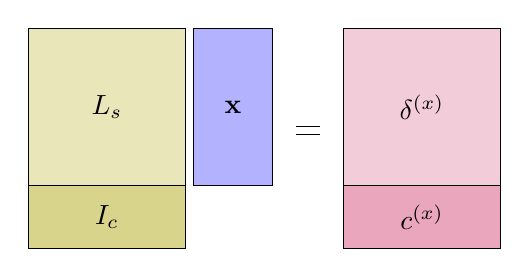
\begin{tikzpicture}
	\filldraw[fill=olive!20!white, draw=black] (0,0) rectangle node{$L_s$} (2,2);
	\filldraw[fill=olive!35!white, draw=black] (0,0) rectangle node{$I_c$} (2,-0.8);
	\filldraw[fill=blue!30!white, draw=black] (2.1,0) rectangle node{$\mathbf{x}$} (3.1,2);
	\draw (3.4, 0.65) -- (3.7, 0.65);
	\draw (3.4, 0.75) -- (3.7, 0.75);
	\filldraw[fill=purple!20!white, draw=black] (4,0) rectangle node{$\delta^{(x)}$} (6,2);
	\filldraw[fill=purple!35!white, draw=black] (4,0) rectangle node{$c^{(x)}$} (6,-0.8);
	\end{tikzpicture}
\end{center}

\noindent neste caso, $I_c$ é a matriz identidade $m \times m$, com zeros à direita (e foi fixado $\omega = 1$ por simplicidade).

A matriz dos coeficientes em \ref{eq:sisrecover} é denominada $\tilde{L}$. Por mais que o sistema tenha mais equações que incógnitas, ele é \textit{full-rank} e possui uma única solução com a utilização do método dos mínimos quadrados:

\begin{equation}\label{eq:leastsqrsol}
\mathbf{\tilde{x}} = \mathop{\mathrm{argmin}}_x \left( \lVert L \mathbf{x} - \delta^{(x)} \rVert^2 + \sum_{j \in C} \omega^2 \lvert x_j - c_j \rvert^2  \right)
\end{equation}

Então, por exemplo, para a mesma malha mostrada anteriormente, caso seja fixada a localização dos vértices $1$ e $5$ (como mostrado na figura \ref{fig:fixedmesh}) temos:

\begin{figure}[ht!]
	\centering
	\includegraphics[width=.6\linewidth]{imagens/cap4/grafofixado.eps}
	\caption{Uma malha triangular com os pontos $1$ e $5$ fixados}
	\label{fig:fixedmesh}
\end{figure}

\noindent e é formada a seguinte matriz $\tilde{L}$:

$$\tilde{L} = \begin{pmatrix}
5 & 0 & -1 & -1 & 0 & 0 & -1 & -1 & -1\\
0 & 3 & 0 & 0 & -1 & -1 & 0 & -1 & 0\\
-1 & 0 & 4 & -1 & 0 & -1 & 0 & -1 & 0\\
-1 & 0 & -1 & 3 & 0 & 0 & 0 & 0 & -1\\
0 & -1 & 0 & 0 & 3 & 0 & -1 & -1 & 0\\
0 & -1 & -1 & 0 & 0 & 3 & 0 & -1 & 0\\
-1 & 0 & 0 & 0 & -1 & 0 & 4 & -1 & -1\\
-1 & -1 & -1 & 0 & -1 & -1 & -1 & 6 & 0\\
-1 & 0 & 0 & -1 & 0 & 0 & -1 & 0 & 3\\
1 & 0 & 0 & 0 & 0 & 0 & 0 & 0 & 0\\
0 & 0 & 0 & 0 & 1 & 0 & 0 & 0 & 0
\end{pmatrix}$$

\noindent e a recuperação das coordenadas absolutas com relação ao eixo-x é feita a partir da resolução do seguinte sistema linear:

$$\begin{pmatrix}
5 & 0 & -1 & -1 & 0 & 0 & -1 & -1 & -1\\
0 & 3 & 0 & 0 & -1 & -1 & 0 & -1 & 0\\
-1 & 0 & 4 & -1 & 0 & -1 & 0 & -1 & 0\\
-1 & 0 & -1 & 3 & 0 & 0 & 0 & 0 & -1\\
0 & -1 & 0 & 0 & 3 & 0 & -1 & -1 & 0\\
0 & -1 & -1 & 0 & 0 & 3 & 0 & -1 & 0\\
-1 & 0 & 0 & 0 & -1 & 0 & 4 & -1 & -1\\
-1 & -1 & -1 & 0 & -1 & -1 & -1 & 6 & 0\\
-1 & 0 & 0 & -1 & 0 & 0 & -1 & 0 & 3\\
1 & 0 & 0 & 0 & 0 & 0 & 0 & 0 & 0\\
0 & 0 & 0 & 0 & 1 & 0 & 0 & 0 & 0
\end{pmatrix} \begin{pmatrix} x_1\\x_2\\x_3\\x_4\\x_5\\x_6\\x_7\\x_8\\x_9\end{pmatrix} = \begin{pmatrix}
-4\\
6\\
-6\\
-20\\
10\\
0\\
10\\
-8\\
12\\
6\\
14
\end{pmatrix}$$

\noindent em que os $9$ primeiros valores da matriz à direita são as $\delta$-coordenadas relativas aos vértices, e os $2$ últimos se referem à localização absoluta dos vértices fixados.

\subsection{Ponderação das $\delta$-coordenadas}
\label{Pondera}

Existem outras formas de se calcular as $\delta$-coordenadas, de forma a se obter melhores qualidades de aproximação. Por exemplo, ao adicionar pesos às arestas de $E$, é possível alterar a forma como um vértice $\mathbf{v_i}$ interage com um vértice vizinho $\mathbf{v_j}$. É possível inclusive modificar o peso de cada aresta de $E$ que parte de $\mathbf{v_i}$ individualmente, de forma que a interação do vértice com cada um de seus vértices vizinhos ocorra de uma maneira singular, dependente da relação entre eles. Desta forma, podemos obter a seguinte fórmula que rege as operações de ponderação das $\delta$-coordenadas:

\begin{equation}
\mathbf{\delta}_i = {c_i} \sum_{j \in N(i)} \mathbf{w}_{ij}(\mathbf{v}_i - \mathbf{v}_j)
\label{eq_forpon}
\end{equation}

\noindent onde $\mathbf{c_i}$ é uma constante particular do vértice $\mathbf{v_i}$ e $\mathbf{w}_{ij}$ é o peso da aresta entre $\mathbf{v_i}$ e $\mathbf{v_j}$.

 Por simplicidade, foi apresentada anteriormente a ponderação média, um método em que o peso de todas as arestas é constante e $\mathbf{c_i}$ depende unicamente do número de vizinhos de $\mathbf{v_i}$. Desta forma, alterações sofridas por um vértice são distribuídas uniformemente entre os vértices vizinhos a ele. A fórmula deste método, como apresentada anteriormente, é: 

\begin{equation}
    \mathbf{\delta}_i = \frac{1}{d_i} \sum_{j \in N(i)} (\mathbf{v}_i - \mathbf{v}_j)
\end{equation}

Outro método utilizado para a ponderação de $\delta$-coordenadas é o uso de pesos cotangentes. Neste método, recomendável para malhas muito irregulares, a ponderação geométrica do somatório se dá com o uso de cotangentes \cite{pinkall:1996}, resultando na seguinte equação:

\begin{equation}
	\mathbf{\delta}_i^c = \frac{1}{|\Omega|} \sum_{j \in N(i)} \frac{1}{2} (\cot \alpha_{ij} + \cot \beta_{ij})(\mathbf{v}_i - \mathbf{v}_j))
\end{equation}

\noindent em que $|\Omega|$ é o tamanho da célula de Voronoi de $i$ e $\alpha_{ij}, \beta_{ij}$ são os dois ângulos opostos à aresta $(i, j)$. Esta ponderação gera os vetores $\mathbf{\delta}_i^c$, que possuem apenas componentes normais (ao contrário das $\mathbf{\delta}$-coordenadas definidas anteriormente, que podem possuir componentes tangenciais e serem não nulas em 1-anéis planares). Porém, os valores das cotangentes podem ser negativos ou possuírem algum outro problema caso os ângulos possuam valores que se aproximem de $\pi$.

Utilizando estes métodos, ou métodos similares, é possível controlar a modificação de malhas e alterar o relacionamento entre vértices, de forma que alterações sejam propagadas pela malha da maneira que o usuário desejar.

\subsection{Molas e malhas dinâmicas}
\label{MD}
Durante o processo de manipulação de malhas é de crucial importância garantir que a nova malha gerada após as transformações da malha original é válida. Existe um número de maneiras de executar estas transformações e, através delas, garantir que a malha final é válida, cada qual com suas vantagens e desvantagens, dentre as quais está o uso de malhas dinâmicas.

\begin{defi}[Malhas Dinâmicas]
    O uso de Malhas Dinâmicas é uma técnica de modelagem em que as posições dos vértices $V$ de uma malha poligonal $M$ são modificadas para atender mudanças de domínio na malha sem que sejam alterados os membros do conjunto $E$. A criação de uma malha dinâmica se dá através da distribuição de molas virtuais em $M$. Estas molas possuem a função de modificar a posição dos membros de $V$ quando ocorrer alguma alteração em $M$ ou no domínio de $M$.\cite{soares2007}
\end{defi}

É possível também adicionar molas internas entre os tetraedros formados por diferentes vértices em malhas tridimensionais triangulares\cite{soares2007}. 
Isso aumenta o controle que temos ao mover uma determinada parte da malha em relação à outras partes.
Algumas precauções devem ser tomadas durante o processo de inserção das molas virtuais para evitar que estas molas adicionadas a $M$ levem a comportamentos indevidos da malha dinâmica, como, por exemplo, uma face da malha possuir área negativa após uma alteração de domínio. Finalmente, é importante ressaltar que uma malha dinâmica pode ser incapaz de lidar com grandes distorções no domínio, uma vez que arestas adicionais não são acrescentadas a $M$. Neste caso, o remalhamento é necessário para produzir uma malha capaz de suportar estas modificações.

Com base nos princípios de malhas dinâmicas, um método para a movimentação das posições de vértices vizinhos de um vértice cuja posição foi modificada em uma malha consiste na modificação do comportamento das arestas de $E$ para que elas atuem como molas. 
Isto é, ao adicionar pesos às arestas de $E$, estas passam a simular o comportamento de molas.
\begin{defi}[Lei de Hooke]
A Lei da Elasticidade de Robert Hooke enuncia que a força necessária para deformar uma mola é diretamente proporcional à deformação sofrida e a constante de elasticidade do material que compõe a mola, de forma que 
\begin{equation}
    \mathbf{\mathcal}F = -kx
\end{equation}
Onde $F$ é a força exercida pela (e a força oposta a $F$ sobre a) mola, $k$ é a constante de elasticidade particular da mola, e $x$ é a deformação sofrida pela mola.
\end{defi}
Submetendo as arestas de $E$ à lei de Hooke, a malha $M$ adota o comportamento de uma malha dinâmica, de forma que quando um vértice é movido, o movimento é transmitidos pelas arestas que, por sua vez, transmitem a força F e provocam alterações nos vértices vizinhos.
Como visto na seção \ref{Pondera}, as $\delta$-coordenadas podem ser ponderadas com base no peso das arestas entre um vértice sendo modificado e seus vizinhos. Utilizando esta técnica e tratando o $k$ particular de cada aresta, ou seja, sua constante de elasticidade, como sendo o peso dela, este valor pode ser manipulado para alterar a forma como os vizinhos são afetados quando um vértice é movido. Por exemplo, $k$ pode ser constante para todos os membros de $E$, e assim todos os vértices vizinhos serão afetados da mesma forma. Outra possibilidade é definir $k$ de forma que a elasticidade de cada aresta seja inversamente proporcional ao seu tamanho. Desta forma, vértices serão mais afetados por transformações de um vizinho mais próximo, enquanto vizinhos mais afastados, ligados por arestas maiores que possuem $k$ menor, irão sofrer transformações mais brandas.

%% Juntei as partes de `usos e tecnicas` e `aplicacoes`

\section{Aplicações e exemplos}\label{LB_matlab}
Como dito anteriormente, a representação pelas $\delta$-coordenadas permitem o encapsulamento de informações locais da superfície. Além disso, as matrizes $L, L_s$ e $D$ utilizadas são esparsas, e computacionalmente mais eficientes em questão de memória e tempo de execução.

Com isso, a modelagem utilizando estas coordenadas possuem algumas vantagens interessantes, que serão exploradas nos próximos tópicos.

\subsection{Representação eficiente de formas}

A primeira grande aplicação das coordenadas diferenciais a ser analisada é a representação eficiente de formas, mesmo ao utilizar informações reduzidas do domínio. Se utilizada uma boa base para representação, é necessária apenas uma parcela da função de base para representar toda a geometria \cite{sorkine2004}.

Desta forma, com apenas informações de conectividade da malha e alguns pontos fixados (denominados vértices âncora), é possível aproximar toda a geometria, a partir da resolução do sistema pelo método dos mínimos quadrados:

\begin{equation}\label{eq:sisrecover2}
\left( \frac{L}{\omega I_{m \times m} | 0} \right) \mathbf{x'} = \begin{pmatrix}
0\\
\omega\ c_{1:m}^{(x)}
\end{pmatrix}
\end{equation}

\noindent em que $c = \{v_1, v_2, \dots, v_m\}$ são os pontos âncora escolhidos como amostra, e $\omega > 0$ é o peso de cada restrição (assim como na equação \ref{eq:sisrecover}).

Da mesma forma que anteriormente, de forma gráfica, para facilitar a visualização do sistema:

\begin{center}
	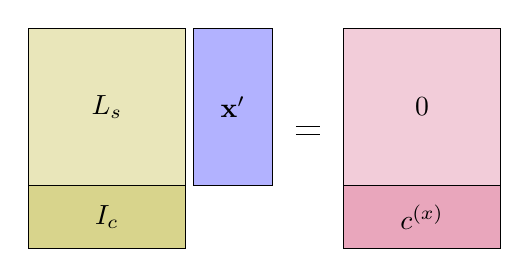
\begin{tikzpicture}
	\filldraw[fill=olive!20!white, draw=black] (0,0) rectangle node{$L_s$} (2,2);
	\filldraw[fill=olive!35!white, draw=black] (0,0) rectangle node{$I_c$} (2,-0.8);
	\filldraw[fill=blue!30!white, draw=black] (2.1,0) rectangle node{$\mathbf{x}'$} (3.1,2);
	\draw (3.4, 0.65) -- (3.7, 0.65);
	\draw (3.4, 0.75) -- (3.7, 0.75);
	\filldraw[fill=purple!20!white, draw=black] (4,0) rectangle node{$0$} (6,2);
	\filldraw[fill=purple!35!white, draw=black] (4,0) rectangle node{$c^{(x)}$} (6,-0.8);
	\end{tikzpicture}
\end{center}

As figuras \ref{fig:ex1rep} e \ref{fig:ex2rep} mostram exemplos de representação de curvas parametrizadas a partir de uma parcela dos pontos originais.

\begin{figure}[htb]
	\centering
	\begin{subfigure}[b]{0.43\textwidth}
		\centering
		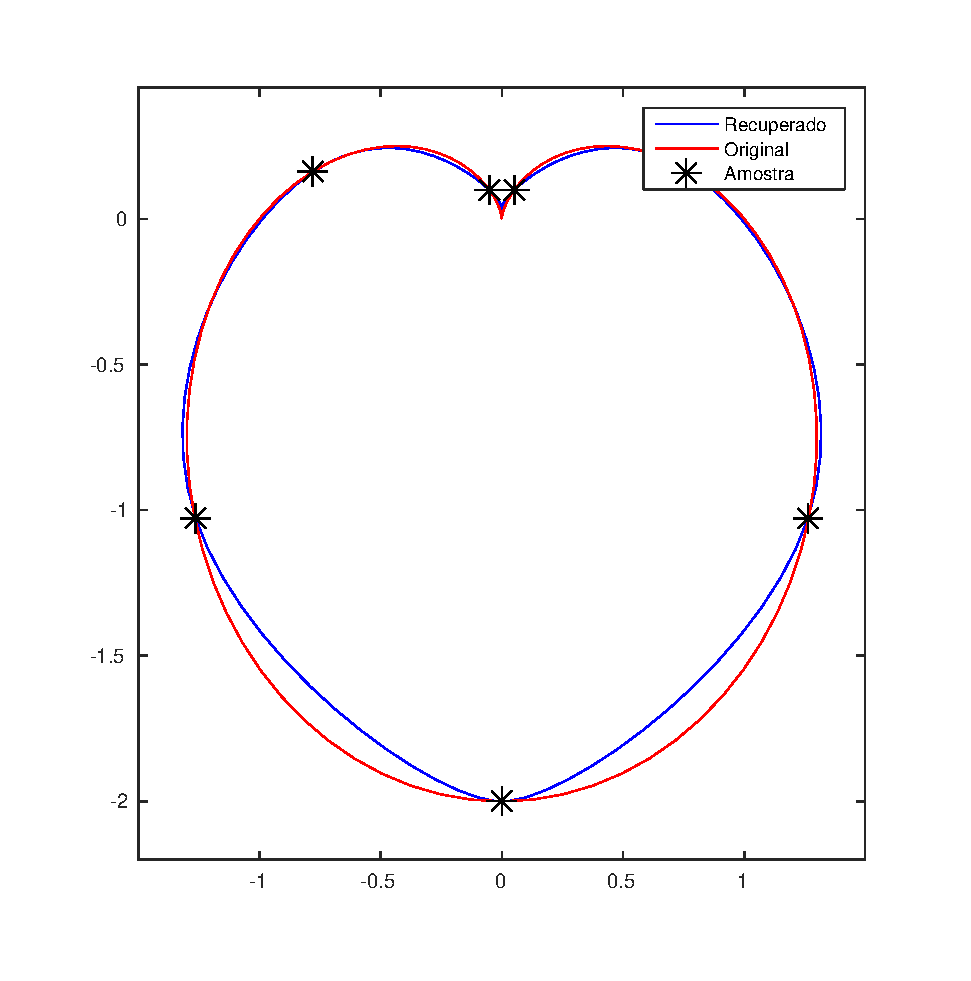
\includegraphics[width=\textwidth]{imagens/cap4/rep_1_8.eps}
		\caption{8 pontos}
		\label{fig:ex11}
	\end{subfigure}
	\hfill
	\begin{subfigure}[b]{0.43\textwidth}
		\centering
		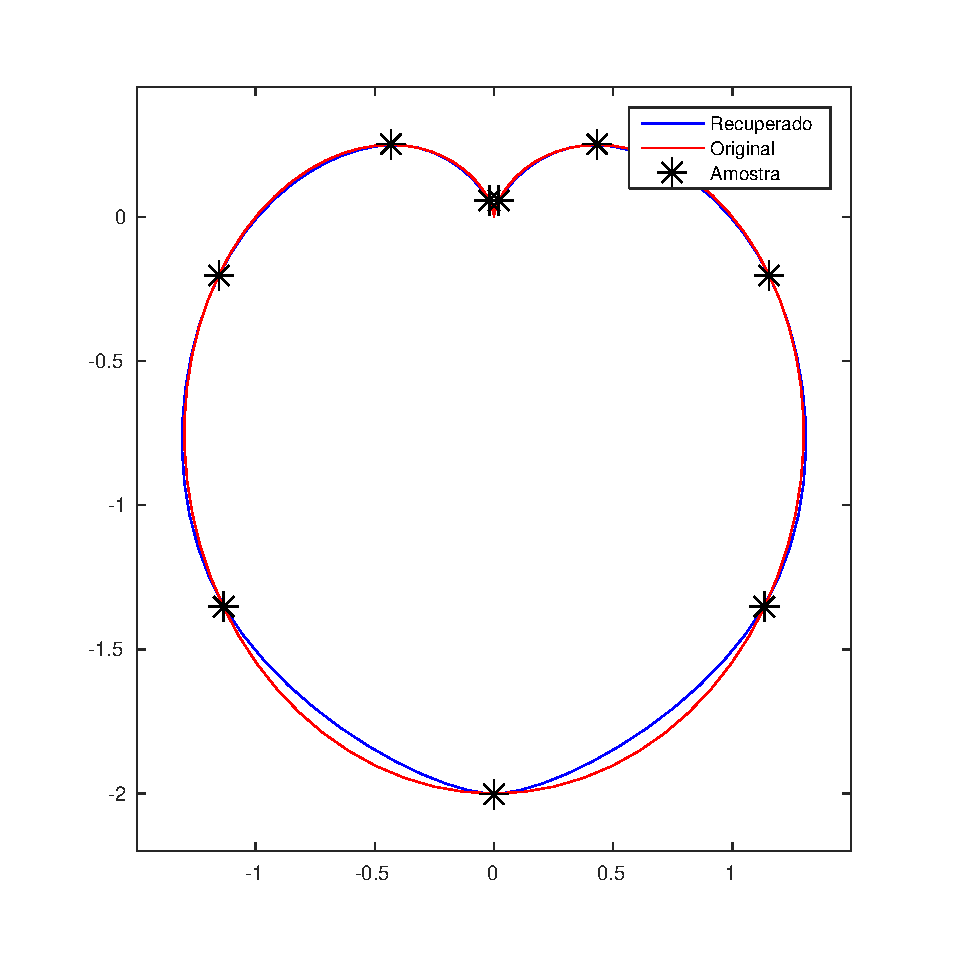
\includegraphics[width=\textwidth]{imagens/cap4/rep_1_10.eps}
		\caption{10 pontos}
		\label{fig:ex14}
	\end{subfigure}
	\hfill
	\begin{subfigure}[b]{0.43\textwidth}
		\centering
		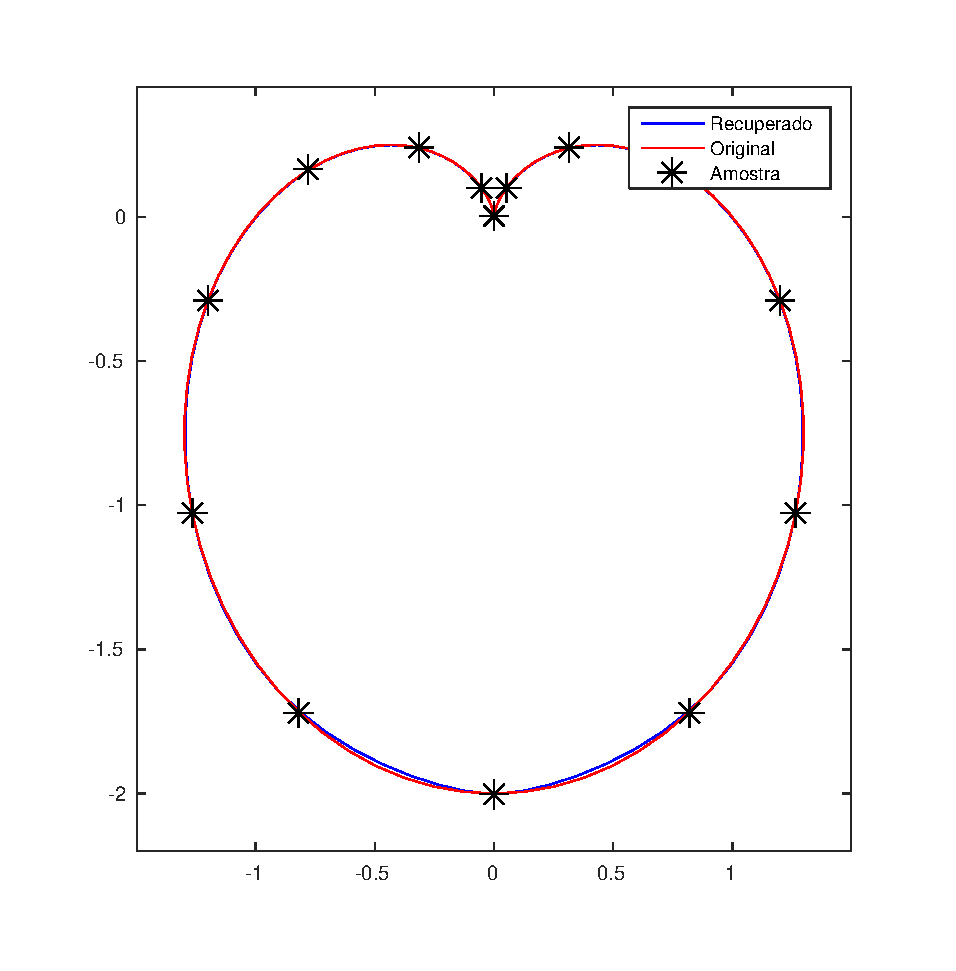
\includegraphics[width=\textwidth]{imagens/cap4/rep_1_15.eps}
		\caption{15 pontos}
		\label{fig:ex12}
	\end{subfigure}
	\hfill
	\begin{subfigure}[b]{0.43\textwidth}
		\centering
		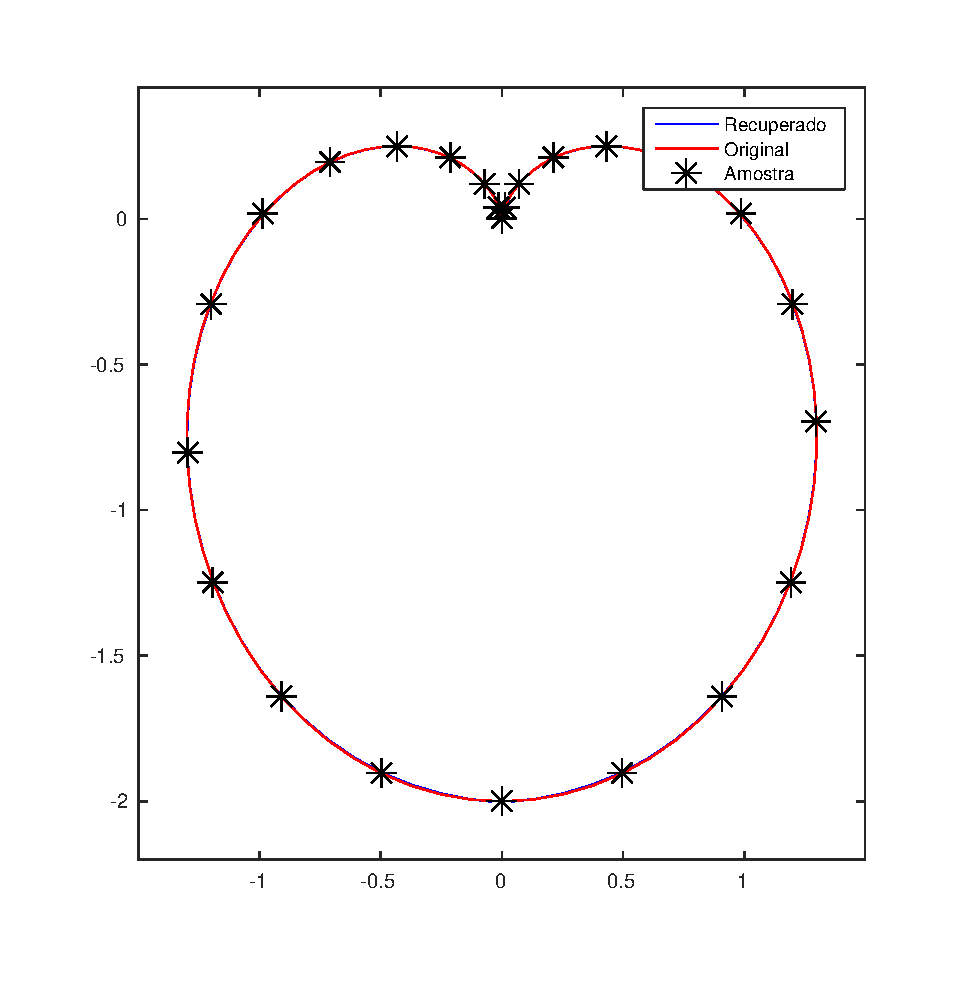
\includegraphics[width=\textwidth]{imagens/cap4/rep_1_25.eps}
		\caption{25 pontos}
		\label{fig:ex13}
	\end{subfigure}
	\caption{Representação da função paramétrica $(x(t), y(t)) = (sin(t) + 0.5 sen(2t), -cos(t) - 0.5 - 0.5 cos(2t))$ utilizando alguns pontos igualmente espaçados como amostra.}
	\label{fig:ex1rep}
\end{figure}


\begin{figure}[htb]
	\centering
	\begin{subfigure}[b]{0.43\textwidth}
		\centering
		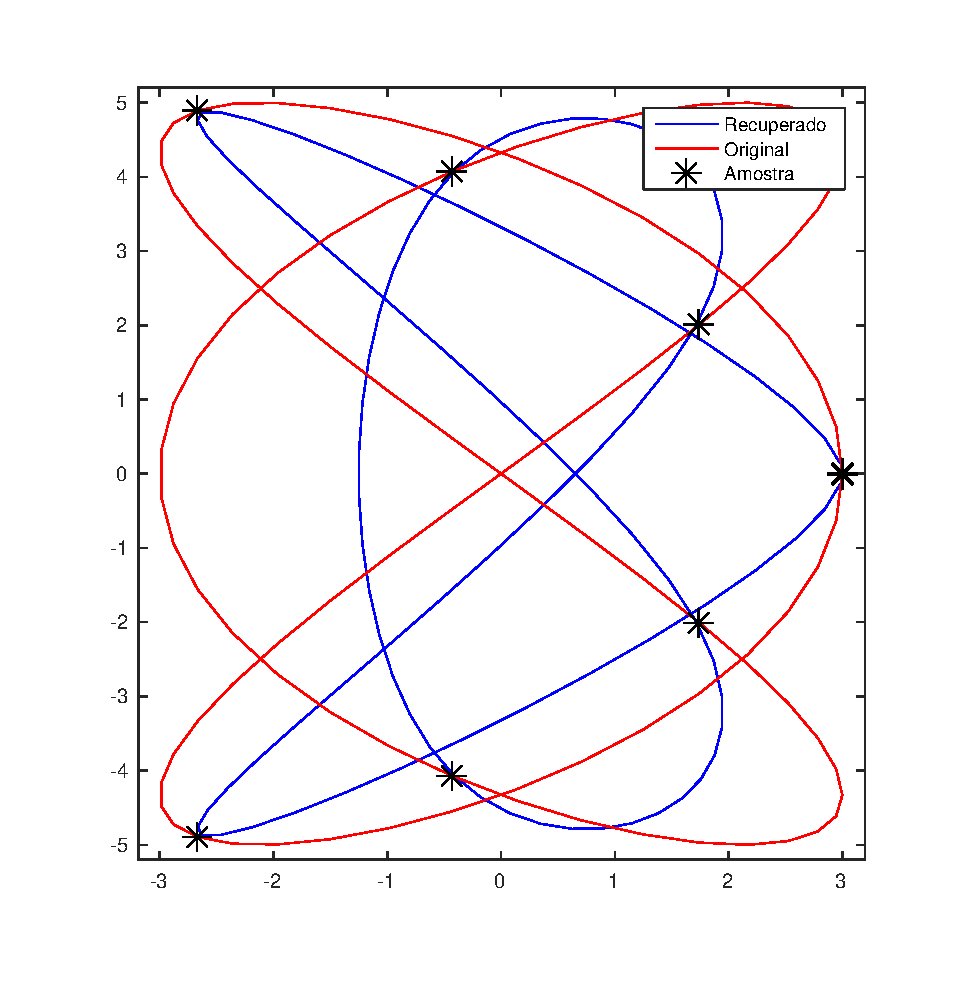
\includegraphics[width=\textwidth]{imagens/cap4/rep_2_8.eps}
		\caption{8 pontos}
		\label{fig:ex21}
	\end{subfigure}
	\hfill
	\begin{subfigure}[b]{0.43\textwidth}
		\centering
		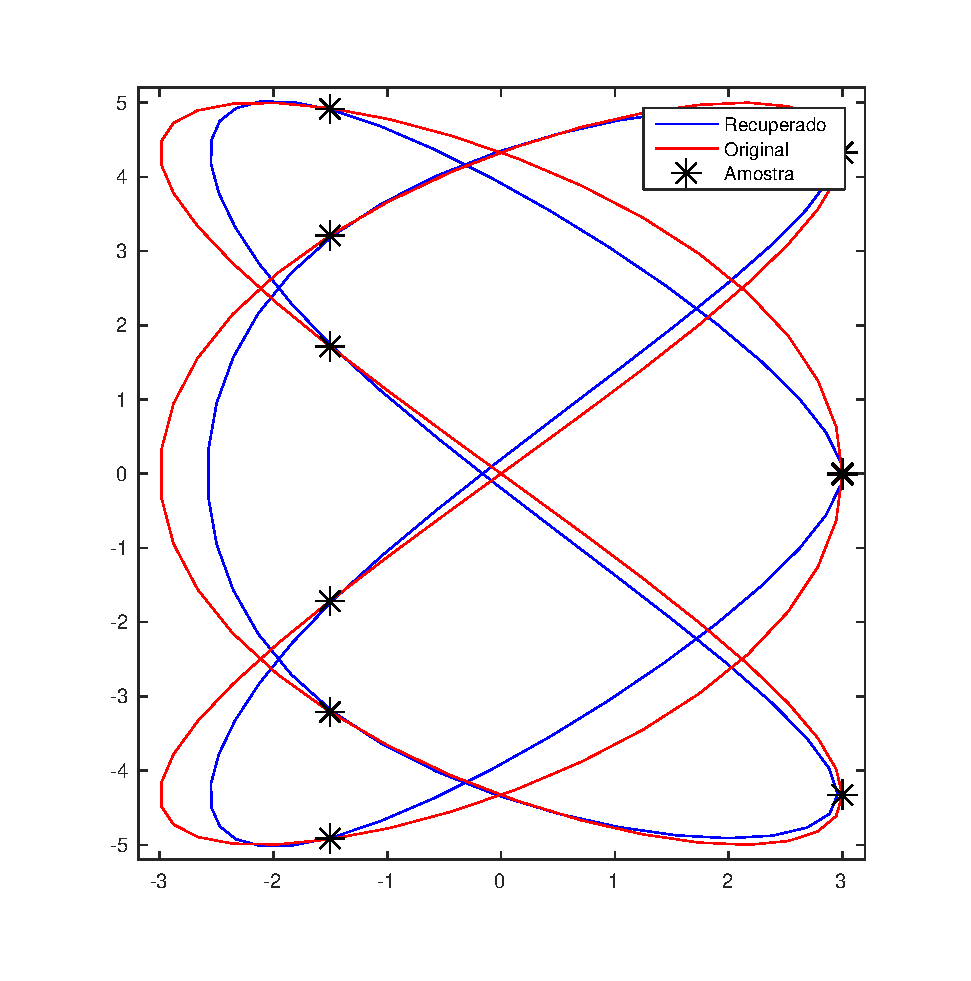
\includegraphics[width=\textwidth]{imagens/cap4/rep_2_10.eps}
		\caption{10 pontos}
		\label{fig:ex24}
	\end{subfigure}
	\hfill
	\begin{subfigure}[b]{0.43\textwidth}
		\centering
		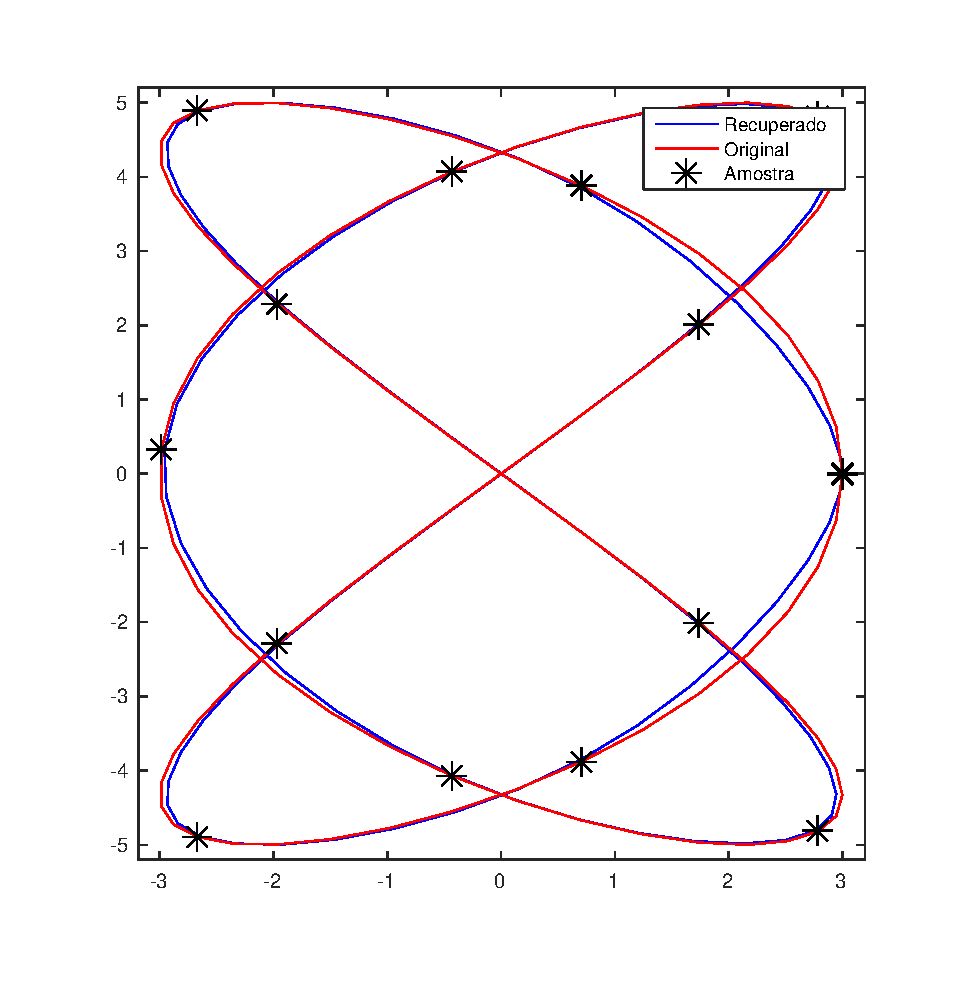
\includegraphics[width=\textwidth]{imagens/cap4/rep_2_15.eps}
		\caption{15 pontos}
		\label{fig:ex22}
	\end{subfigure}
	\hfill
	\begin{subfigure}[b]{0.43\textwidth}
		\centering
		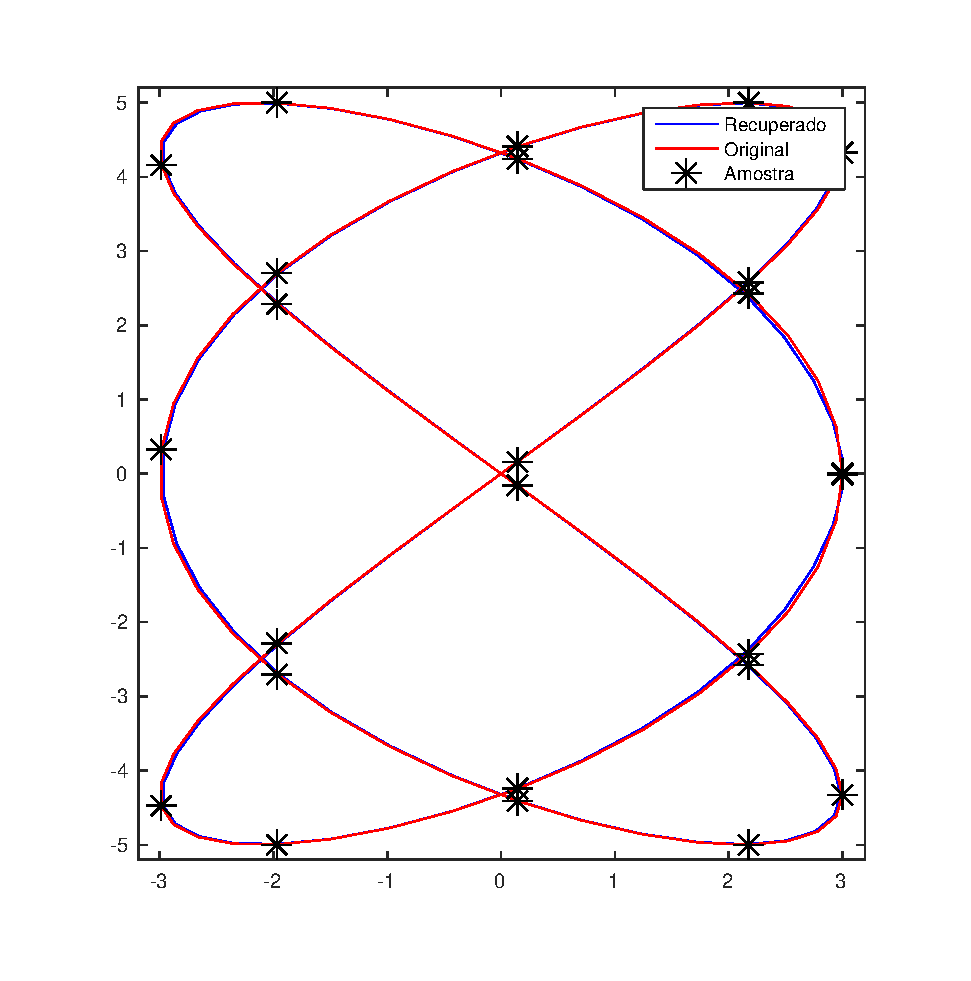
\includegraphics[width=\textwidth]{imagens/cap4/rep_2_25.eps}
		\caption{25 pontos}
		\label{fig:ex23}
	\end{subfigure} %[3 * cos(3 * t); 5 * sin(2 * t)]';
	\caption{Representação da função paramétrica $(x(t), y(t)) = (3 cos(3t), 5sen(2t))$ utilizando alguns pontos igualmente espaçados como amostra.}
	\label{fig:ex2rep}
\end{figure}

Um exemplo de representação de superfícies pode ser visto na figura \ref{fig:ex3rep}, também utilizando alguns pontos igualmente espaçados como amostra (âncora).

\begin{figure}[H]
	\centering
	\begin{subfigure}[b]{0.48\textwidth}
		\centering
		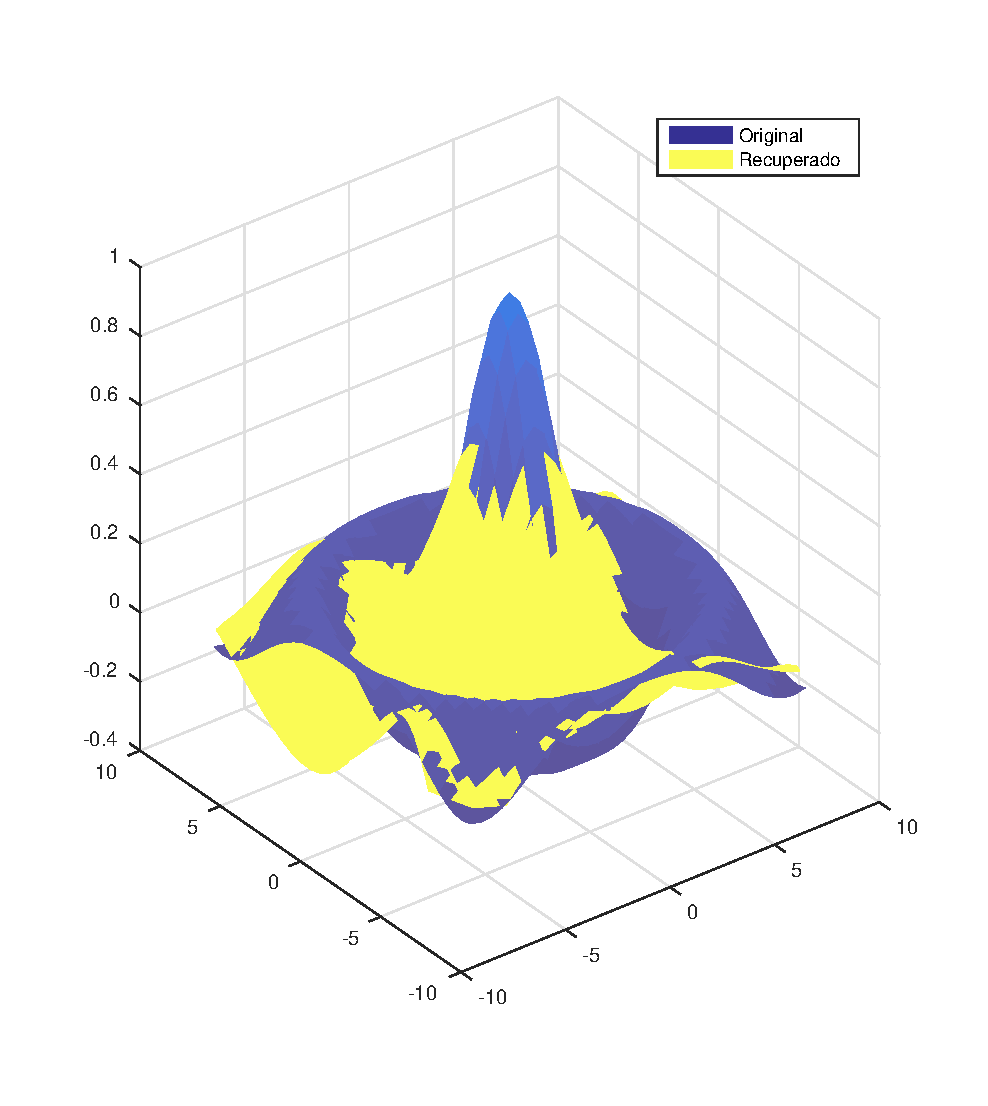
\includegraphics[width=\textwidth]{imagens/cap4/rep3_50.eps}
		\caption{50 pontos}
		\label{fig:ex31}
	\end{subfigure}
	\hfill
	\begin{subfigure}[b]{0.48\textwidth}
		\centering
		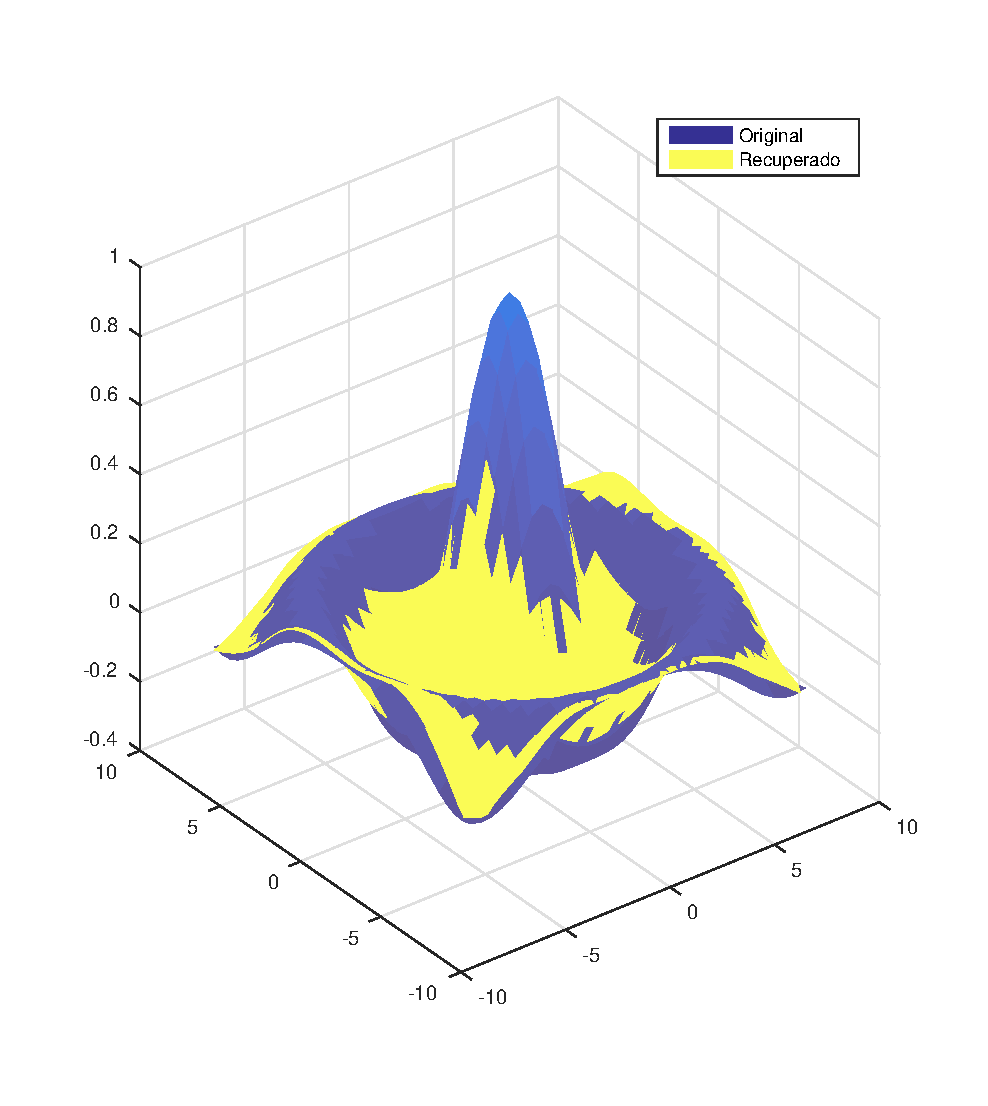
\includegraphics[width=\textwidth]{imagens/cap4/rep3_200.eps}
		\caption{200 pontos}
		\label{fig:ex32}
	\end{subfigure}
	\caption{Representação da função $z(x, y) = \frac{sen (\sqrt{x^2 + y^2})}{\sqrt{x^2 + y^2}}$ utilizando alguns pontos igualmente espaçados como amostra.}
	\label{fig:ex3rep}
\end{figure}

Outro exemplo em espaços tridimensionais pode ser visto na seguinte malha da figura \ref{fig:ex4rep}, utilizando alguns pontos (com índices igualmente espaçados) como âncoras:

\begin{figure}[H]
	\centering
	\begin{subfigure}[b]{0.47\textwidth}
		\centering
		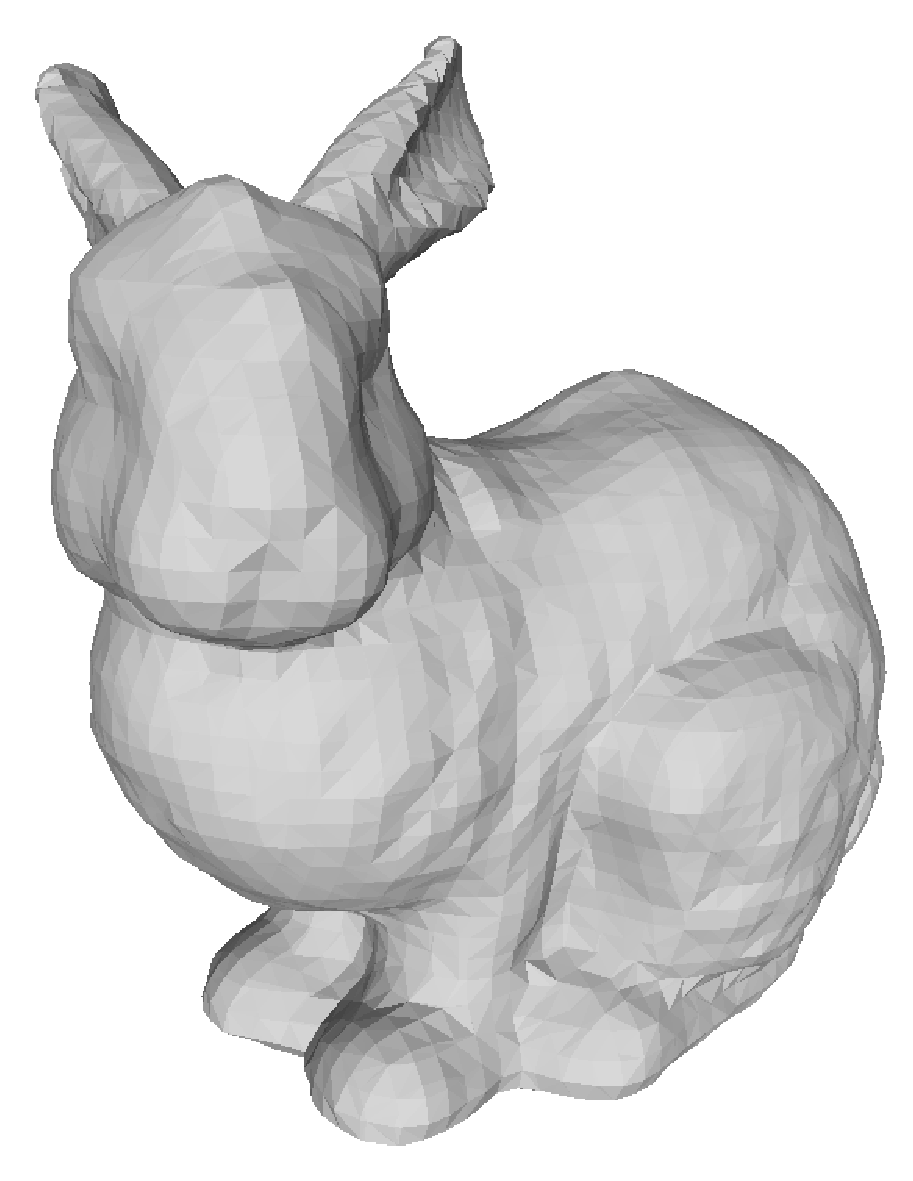
\includegraphics[width=\textwidth]{imagens/cap4/bunny_all.eps}
		\caption{Malha original}
		\label{fig:ex41}
	\end{subfigure}
	\hfill
	\begin{subfigure}[b]{0.47\textwidth}
	\centering
	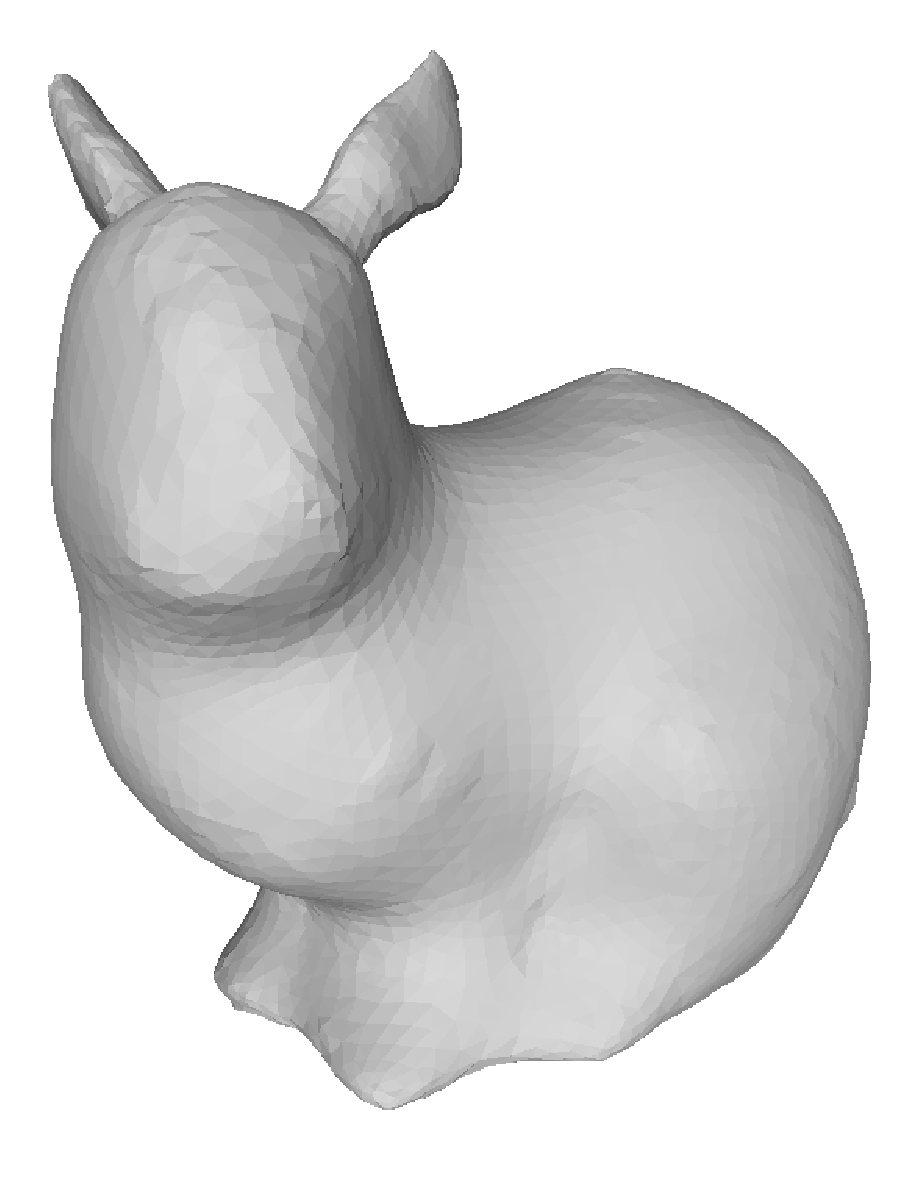
\includegraphics[width=\textwidth]{imagens/cap4/bunny_10.eps}
	\caption{10\% dos pontos}
	\label{fig:ex42}
	\end{subfigure}
	\\
	\begin{subfigure}[b]{0.47\textwidth}
		\centering
		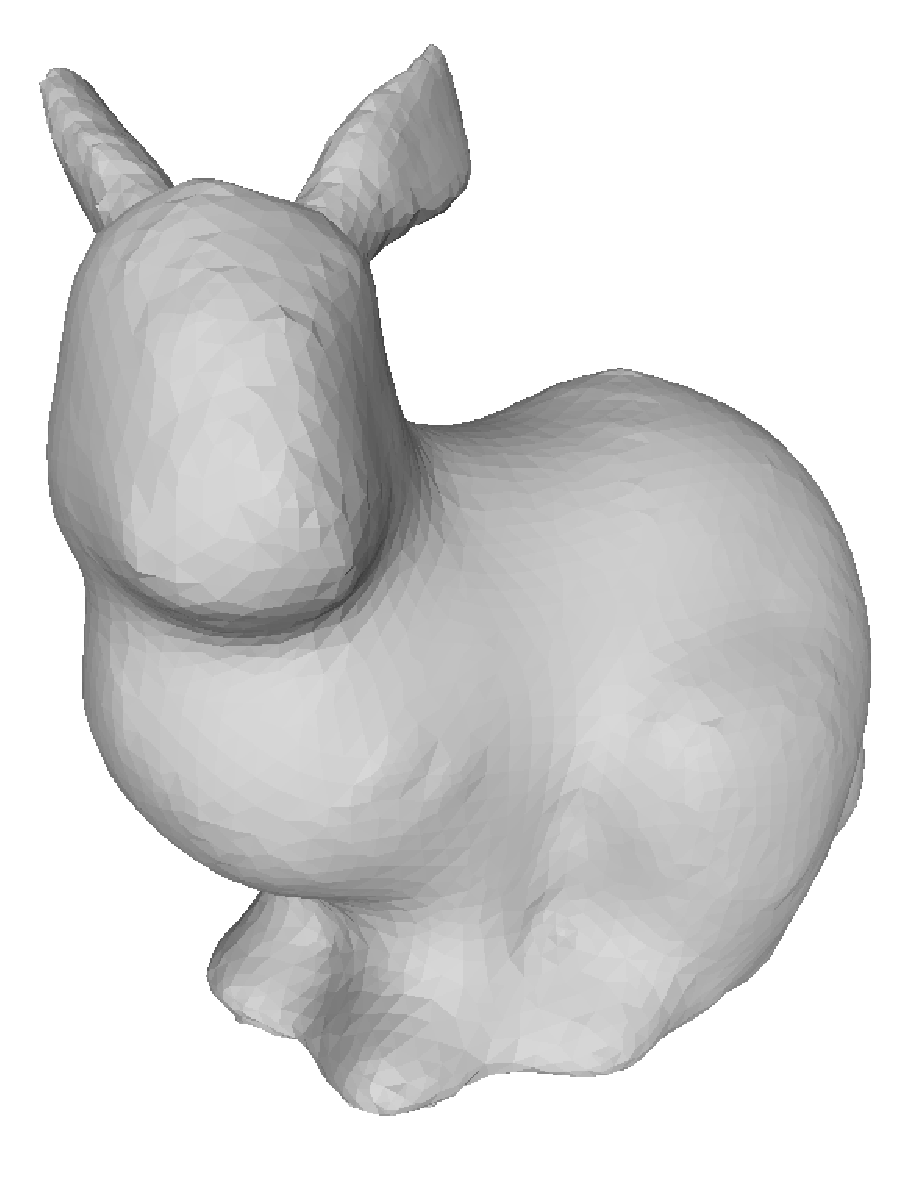
\includegraphics[width=\textwidth]{imagens/cap4/bunny_30.eps}
		\caption{10\% dos pontos}
		\label{fig:ex43}
	\end{subfigure}
	\hfill
	\begin{subfigure}[b]{0.47\textwidth}
		\centering
		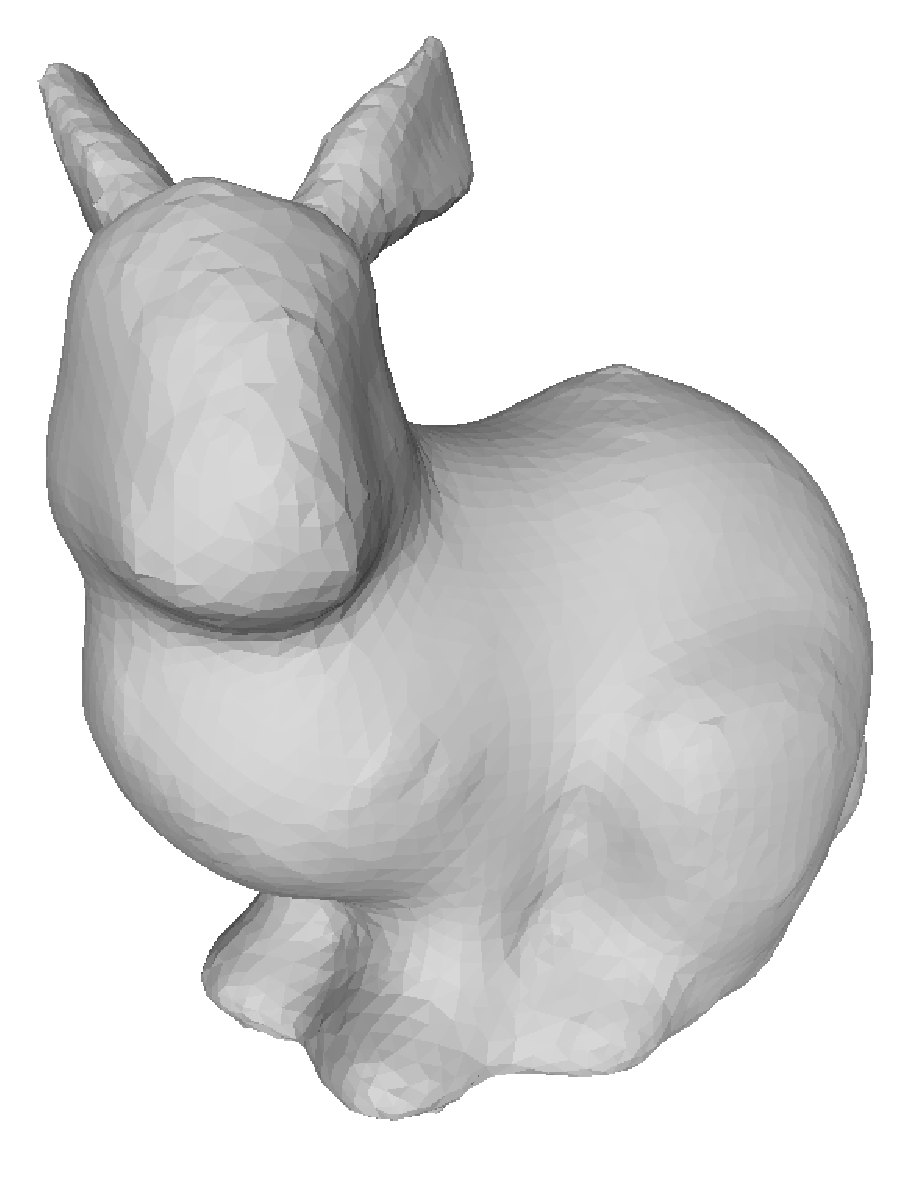
\includegraphics[width=\textwidth]{imagens/cap4/bunny_50.eps}
		\caption{50\% dos pontos}
		\label{fig:ex44}
	\end{subfigure}
	\caption{Representação da malha de um coelho, utilizando apenas uma amostra dos pontos originais como âncoras.}
	\label{fig:ex4rep}
\end{figure}


Nesta figura \ref{fig:ex4rep}, pode-se perceber que alguns detalhes visualmente impactantes do coelho (como o nariz e as pernas) são formados por poucos pontos, e que se estes não forem escolhidos como âncora, os detalhes podem ser perdidos.

\subsection{Edição de malhas}

Outra aplicação interessante das coordenadas diferenciais é a edição de malhas.

Para a edição de alguns vértices da malha, é feito algo similar à reconstrução mostrada anteriormente - porém, além dos pontos âncora, também serão adicionadas restrições dos vértices a serem editados.

Ou seja, além dos $m$ pontos $c = \{v_1, \dots, v_m\}$, são escolhidos $a$ pontos de índices $\{m+1, m+2, \dots, m+a\}$ denominados $e = \{v_{m+1}, v_{m+2}, \dots, v_{m+a}\}$ (novamente, por simplicidade, os pontos são indexados nas primeiras posições, logo após os pontos âncora), e adicionadas as restrições do tipo:

\begin{align}
\mathbf{v}_i &= \mathbf{c}_i, &i \in \{1, \dots, m\}\\
\mathbf{v}_j &= \mathbf{e}_j, &j \in \{m+1, \dots, m+a\}
\end{align}

\noindent e, matricialmente, o sistema pode ser escrito como:

\begin{equation}\label{eq:sisrecoveredi}
\left( \frac{L}{\omega I_{(m+a) \times (m+a)} | 0} \right) \mathbf{x'} = \begin{pmatrix}
\delta^{(x)}\\
\omega\ c_{1:m}^{(x)}\\
\omega\ e_{1:a}^{(x)}
\end{pmatrix}
\end{equation}

Ou seja, De forma gráfica, o sistema a ser resolvido para a edição pode ser visto como:

\begin{center}
	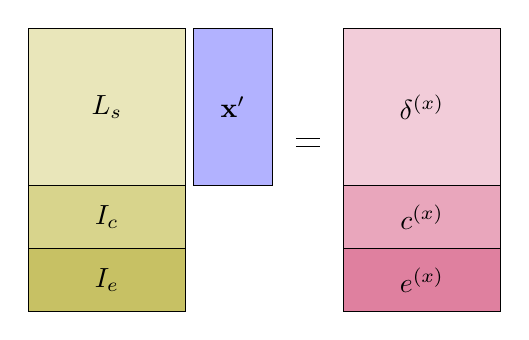
\begin{tikzpicture}
	\filldraw[fill=olive!20!white, draw=black] (0,0) rectangle node{$L_s$} (2,2);
	\filldraw[fill=olive!35!white, draw=black] (0,0) rectangle node{$I_c$} (2,-0.8);
	\filldraw[fill=olive!50!white, draw=black] (0,-0.8) rectangle node{$I_e$} (2,-1.6);
	\filldraw[fill=blue!30!white, draw=black] (2.1,0) rectangle node{$\mathbf{x'}$} (3.1,2);
	\draw (3.4, 0.50) -- (3.7, 0.50);
	\draw (3.4, 0.60) -- (3.7, 0.60);
	\filldraw[fill=purple!20!white, draw=black] (4,0) rectangle node{$\delta^{(x)}$} (6,2);
	\filldraw[fill=purple!35!white, draw=black] (4,0) rectangle node{$c^{(x)}$} (6,-0.8);
	\filldraw[fill=purple!50!white, draw=black] (4,-0.8) rectangle node{$e^{(x)}$} (6,-1.6);
	\end{tikzpicture}
\end{center}

Como é utilizado o método dos mínimos quadrados para a resolução dos sistemas, talvez aconteça alguns erros de precisão. Assim, para minimizar estas falhas, após se encontrar a solução do sistema, pode-se conferir alguns pontos (ou seja, o algoritmo pode, após encontrar os pontos pelo sistema, forçar com que $v'_i = v_i$, para alguns $i$, para que pelo menos estes pontos não sofram erros de precisão).

\begin{figure}[ht!]
	\centering
	\begin{subfigure}[b]{0.45\textwidth}
         \centering
         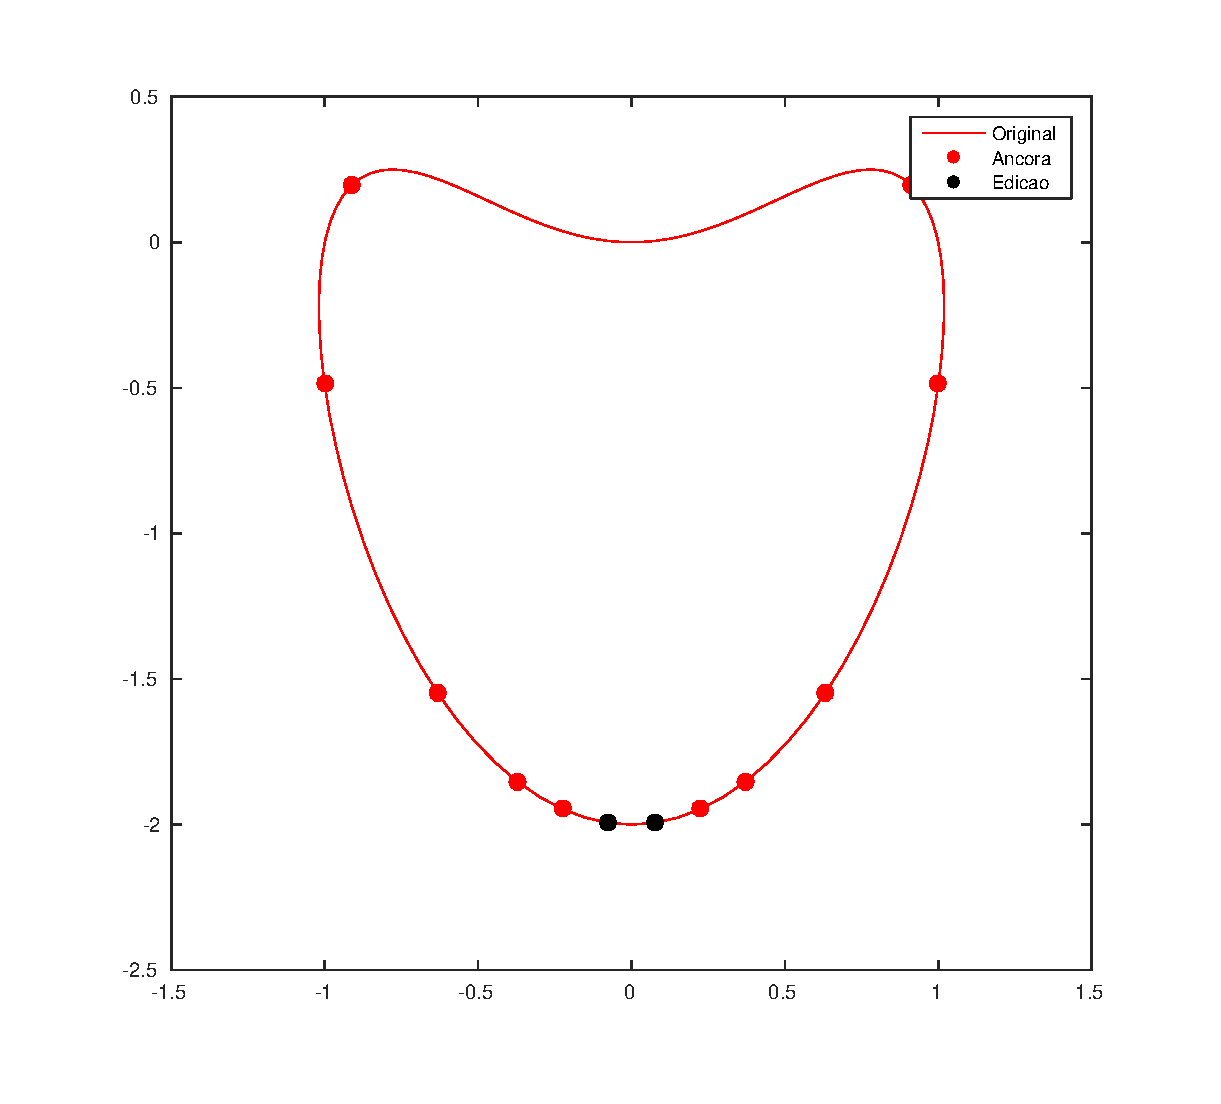
\includegraphics[width=\textwidth]{imagens/cap4/malhaoriginal.eps}
         \caption{Malha original}
         \label{fig:meshorigiedit}
     \end{subfigure}
     \hfill
     \begin{subfigure}[b]{0.45\textwidth}
         \centering
         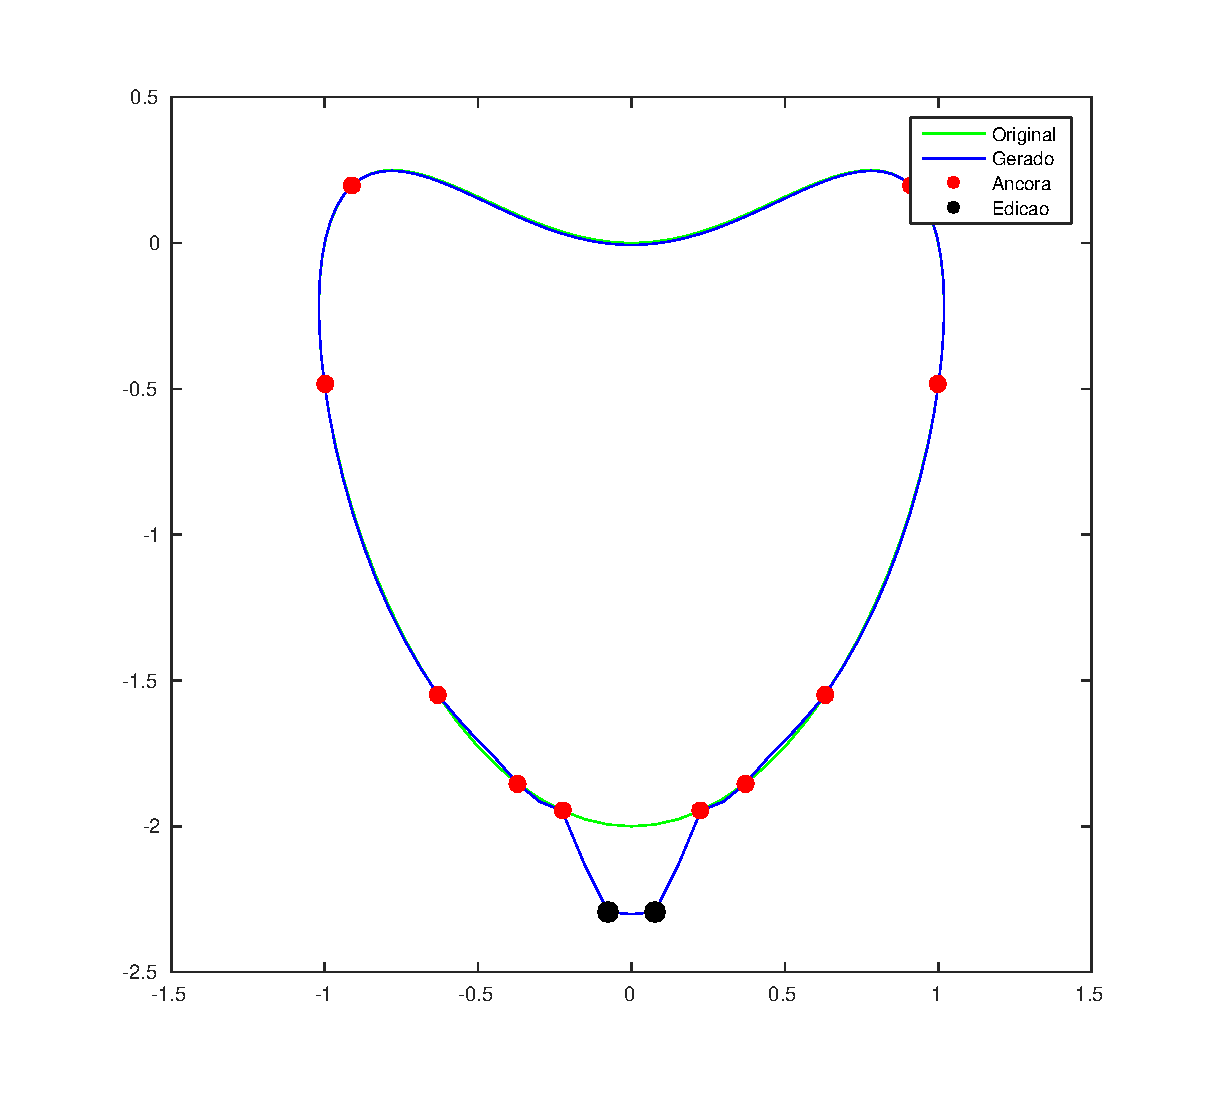
\includegraphics[width=\textwidth]{imagens/cap4/malhaedicao.eps}
         \caption{Malha editada}
         \label{fig:mesheditededit}
     \end{subfigure}
     \caption{Malha antes (\ref{fig:meshorigiedit}) e após edição (\ref{fig:mesheditededit}). Os pontos em vermelho são os pontos de âncora, e os pontos em preto são os editados.}
    \label{fig:editedmesh}
\end{figure}

Este processo pode ser aplicado em malhas tridimensionais, estendendo o sistema de duas $\delta$-coordenadas para três. Ou seja, através da resolução de mais um sistema similar ao exibido acima é possível editar malhas 3D através dos mesmos princípios utilizados para a edição de malhas 2D.  

Além de deformações, também é possível realizar outros tipos de edição, que são discutidas em \cite{sorkine2006}, como inserir marcas d'água, interpolar e suavizar malhas, que não serão discutidos neste livro.



\section{Lista de Exercícios}\label{LB_ListaEx}
\begin{enumerate}
    \item Modelagem geométrica e o uso de malhas poligonais são uma parte intrínseca da computação gráfica. Com uma gama de aplicações e variados usos, a maior parte da humanidade já interagiu com malhas de alguma forma. Sendo assim, quais são alguns destes usos? Procure também encontrar uma malha que você possa manipular de alguma forma. 
    
    \item Construa a matriz de adjacência para uma pirâmide de base quadrada.
    
    \item Construa a matriz de adjacência do exercício anterior em Matlab/Octave.
    
    \item Gere um código em Matlab/Octave que receba uma matriz de adjacências e calcule o laplaciano topológico $L_s$.
    
    \item Gere um código em Matlab/Octave que calcule as $\delta$-coordenadas (com a ponderação padrão vista em \ref{eq_delta}), a partir das coordenadas cartesianas e da matriz de adjacências.
    
    \item Em softwares de visualização de malhas com interação do usuário, é fundamental que o tempo de processamento seja pequeno. Quais as vantagens das matrizes $L$, $L_s$ e $D$ vistas anteriormente em questão de eficiência computacional?
    
    \item Para a representação de formas, é necessário possuir informações de conectividade da malha, como a matriz de adjacências. Como é possível gerar a matriz de adjacência, caso se saiba que a malha é a representação de:
    
\begin{enumerate}
    \item Curva aberta contínua no $\mathbb{R}^2$, em que $v_i \approxeq v(t)$, e os índices estão corretamente ordenados;
    
    \item Curva fechada contínua no $\mathbb{R}^2$, em que $v_i \approxeq v(t)$, e os índices estão corretamente ordenados;
\end{enumerate}

    \item Na seção \ref{LB_matlab}, os pontos âncora foram selecionados como pontos igualmente espaçados. Sugira alguma outra forma para coletá-los, e analise brevemente sua eficiência de representação.

    \item Como visto na seção \ref{Pondera}, alguns dos métodos utilizados para ponderação das $\delta$-coordenadas incluem o uso de pesos cotangentes ou pesos relativos ao número de vizinhos de um vértice. Quais são alguns outros métodos que podem ser utilizados para a ponderação de $\delta$-coordenadas ponderadas?

\end{enumerate}

\subsection{Resoluções}
\begin{enumerate}
    \item De fato, existe um grande número de áreas que utilizam malhas poligonais, desde animação através de computação gráfica, aplicações para decoração de imóveis e arquitetura, modelos computacionais de jogos virtuais, reconhecimento de faces e inúmeras outras aplicações. Também é possível encontrar em diversos repositórios na internet malhas que podem ser carregadas em aplicações que permitem desde a movimentação de câmeras para observação da malha até manipulação direta como torcer, esticar e deformar a malha em geral.
    
    \item Uma possível matriz de adjacência para uma pirâmide em que os pontos 1, 2, 3 e 4 compõe a base é:

$$P = \begin{pmatrix}
0 & 1 & 1 & 0 & 1\\
1 & 0 & 0 & 1 & 1\\
1 & 0 & 0 & 1 & 1\\
0 & 1 & 1 & 0 & 1\\
1 & 1 & 1 & 1 & 0\\
\end{pmatrix}$$

Para transformar essa matriz de adjacência na matriz de uma malha triangular seria necessário adicionar uma aresta entre os pontos 2 e 3 ou 1 e 4.

    \item Vide códigos \textit{geraAdjacenciaPadrao.m} e \textit{geraAdjacenciaPiramide.m}.

    \item Vide código \textit{geraLaplaciano.m}.
    
    \item Vide códigos \textit{geraPesosPadrao.m} e \textit{geraDeltaCoords.m}.

    \item As matrizes descritas são esparsas, o que permite a utilização de algoritmos e estruturas de dados especificas. Além disso, também é possível aplicar algumas decomposições de resolução de sistemas linear (como a decomposição de \textit{Cholesky}) para obter uma maior eficiência.
    
    \item 
    \begin{enumerate}
        \item Caso a malha represente uma curva, e os índices dos nós estejam ordenados conforme o tempo, basta ligar cada vértice $i$ com o predecessor $i-1$ e sucessor $i+1$, para todo $i \in \{2, \dots, n-1\}$. Os extremos (primeiro e último vértices) devem ser tratados a parte: como a curva é aberta, o vértice $1$ está ligado apenas com o $2$, e o vértice $n$ está somente conectado com o $n-1$.
        
        \item Similarmente ao item anterior, basta ligar cada vértice $i$ com o predecessor $i-1$ e sucessor $i+1$, para todo $i \in \{2, \dots, n-1\}$. Porém, como a curva é fechada, além das conexões citadas anteriormente, os vértices $1$ e $n$ também são conectados.
    \end{enumerate}
    
    \item Existem várias sugestões, como pegar os vértices com maior e menor curvatura (podem dar uma melhor representação de curvas), pontos aleatórios (podem ser probabilisticamente melhores ou piores que igualmente espaçados) ou escolher iterativamente os vértices de maneira gulosa (de forma a minimizar a função de erro do método dos mínimos quadrados, que pode ser superior às outras formas discutidas anteriormente).
    
    \item Existem diversas possibilidades para a ponderação de $\delta$-coordenadas. A equação \ref{eq_forpon} descreve a ponderação através dos termos $\mathbf{c_i}$ e $\mathbf{w_{ij}}$, ou seja, alterando estes termos é possível utilizar uma infinidade de métodos de ponderação diferentes. Por exemplo, como mencionado na seção \ref{MD} é possível fazer com que o peso de cada aresta $\mathbf{w_{ij}}$ seja inversamente proporcional ao seu tamanho, isto é, a distância entre $\mathbf{v_i}$ e $\mathbf{v_j}$.
    
\end{enumerate}


%\markboth{Modelagem Utilizando Operadores Diferenciais}{Reconstrução de Superfícies Lineares por Partes}
%\section{Reconstrução de Superfícies Lineares por Partes}\label{proc_recsup}
